\subsubsection{StackGres mit Citus}
\begin{flushleft} 
    StackGres ist eine \Gls{PostgreSQL}-Implementation die dafür vorgesehenen ist, in einem Kubernetes Cluster betrieben zu werden.
\end{flushleft} 
\begin{flushleft}
    An sich wäre StackGres nur eine Implementation von Patroni in Kubernetes inkl. Load Balancer.\\
    Nun kommt das Citus-Plugin ins Spiel, welches aus einer jeden monolithischen, klassischen \Gls{PostgreSQL Cluster} eine Distributed SQL Umgebung macht.
\end{flushleft}
\begin{flushleft}
    Citus Data, der Entwickler von Citus, wiederum ist in den Microsoft-Konzern eingebettet.
\end{flushleft}
\begin{flushleft}
    \paragraph{Core-Features}
    Die wichtigsten Features von StackGres sind \cite{G3XQA8PI}:
    \begin{itemize}
        \item k8s Integration
        \item Deklaratives k8s CRD
        \item Automatische Backups
        \item Grafana und Prometheus integration
        \item Management Web Konsole
        \item Erweiterte Replikationsmöglichkeiten
        \item Integriertes Pooling
        \item Integrierter Proxy
    \end{itemize}
\end{flushleft}
\begin{flushleft}
    \paragraph{Replikation}
    StackGres bietet asynchrone und synchrone Replikation, Gruppenreplikation sowie kaskadierende Replikation an.
\end{flushleft}
\begin{flushleft}
    Citus bietet sein eigenes Modell mit dem Sharding an.
\end{flushleft}
\begin{flushleft}
    \paragraph{Proxy}
    StackGres hat den Proxy bereits mit envoy \cite{QAGSHVBL} implementiert.
\end{flushleft}
\begin{flushleft}
    \paragraph{Pooling}
    PgBounder \cite{ATBELZ2X} ist bereits integriert, es braucht also keinen weiteren \Gls{Connection Pooler}.
\end{flushleft}
\begin{flushleft}
    \paragraph{API / Skripte}
    StackGres wird primär über YAML-Files und Kubernetes gesteuert, bietet aber eine eigene API an.
\end{flushleft}
\begin{flushleft}
    Citus bietet ebenfalls eine eigene API, mit der Citus vollständig verwaltet werden kann.
\end{flushleft}
\begin{flushleft}
    \paragraph{Architektur}
    \begin{flushleft}
        \subparagraph{StackGres}
        StackGres packt \Gls{PostgreSQL}, Patroni, PgBouncer und envoy in einen \Gls{Kubernetes} Pod:
        \begin{figure}[H]
            \centering
            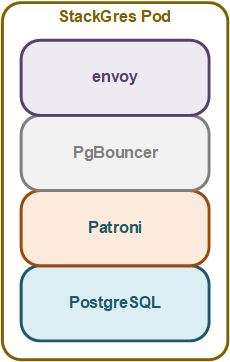
\includegraphics[width=0.4\linewidth]{source/implementation/evaluation/postgresql_ha_solutions/stackgres/stackgres_pod_architecture}
            \caption{Stackgres - Grundarchitektur}
            \label{fig:stackgres_pod_architecture}
        \end{figure}
    \end{flushleft}
    \begin{flushleft}
        \subparagraph{Citus Coordinator und Workers}
        Citus arbeitet mit einem Coordinator-Node, der jedes Query analysiert und an einen Worker-Node weitergibt.\\
        Die unten stehende Grafik zeigt diese Architektur auf:
        \begin{figure}[H]
            \centering
            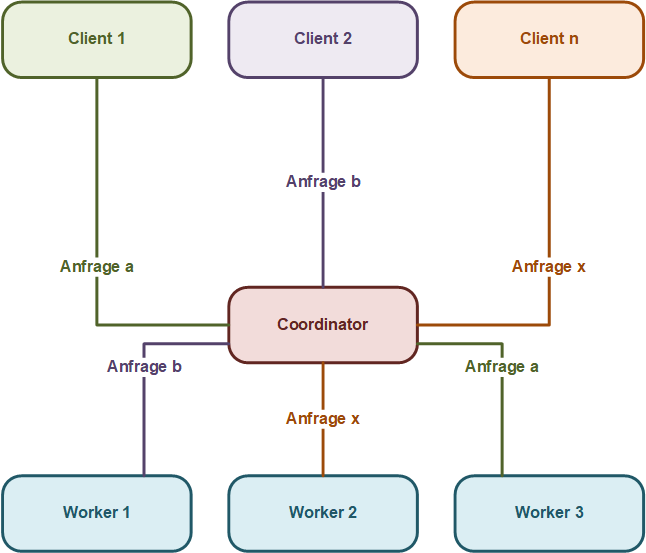
\includegraphics[width=0.75\linewidth]{source/implementation/evaluation/postgresql_ha_solutions/stackgres/citus_coordinator_worker}
            \caption{Citus - Coordinator und Workers}
            \label{fig:citus_coordinator_worker}
        \end{figure}
    \end{flushleft}
    \begin{flushleft}
        \subparagraph{Citus Sharding}
        \label{subpar:citus_sharding}
        Citus bietet zwei Sharding-Modelle an.
        \begin{flushleft}
            \textbf{Row-based sharding}\\
            Beim diesen Sharding werden Tabellen anhand einer Distribution Column aufgeteilt \cite{2Y5FA36C, FDUUL9IM}:
            \begin{figure}[H]
                \centering
                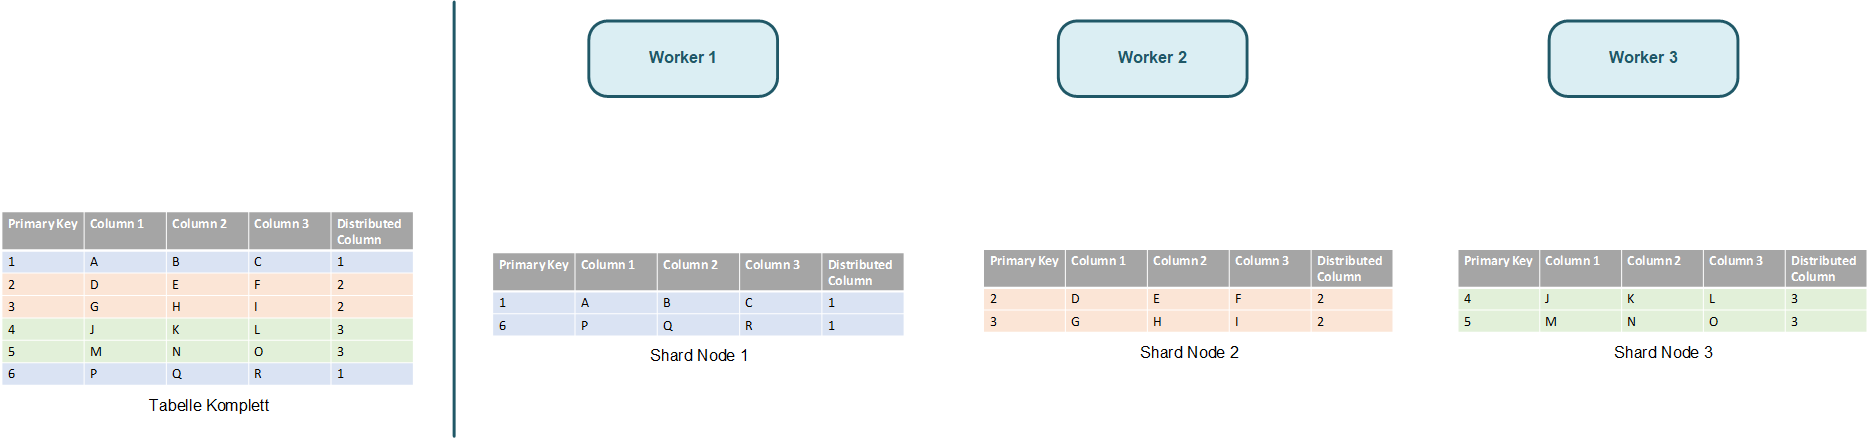
\includegraphics[width=0.8\linewidth]{source/implementation/evaluation/postgresql_ha_solutions/stackgres/citus_row-based-sharding}
                \caption{Citus - Row-Based-Sharding}
                \label{fig:citus_row-based-sharding}
            \end{figure}
        \end{flushleft}
        \begin{flushleft}
            \textbf{Schema-based sharding}\\
            Beim Schema-based sharding werden die Tabellen horizontal partitioniert oder gleich ganze Tabellen in den Shard gepackt.
            Die Shards werden dabei nach Schema aufgeteilt, wobei ein Schema auf einem Node verbleibt.
            Dadurch braucht es im Prinzip keine Anpassung an den Tabellen und Applikationen.
            Das Prinzip wird unten aufgezeigt:
            \begin{figure}[H]
                \centering
                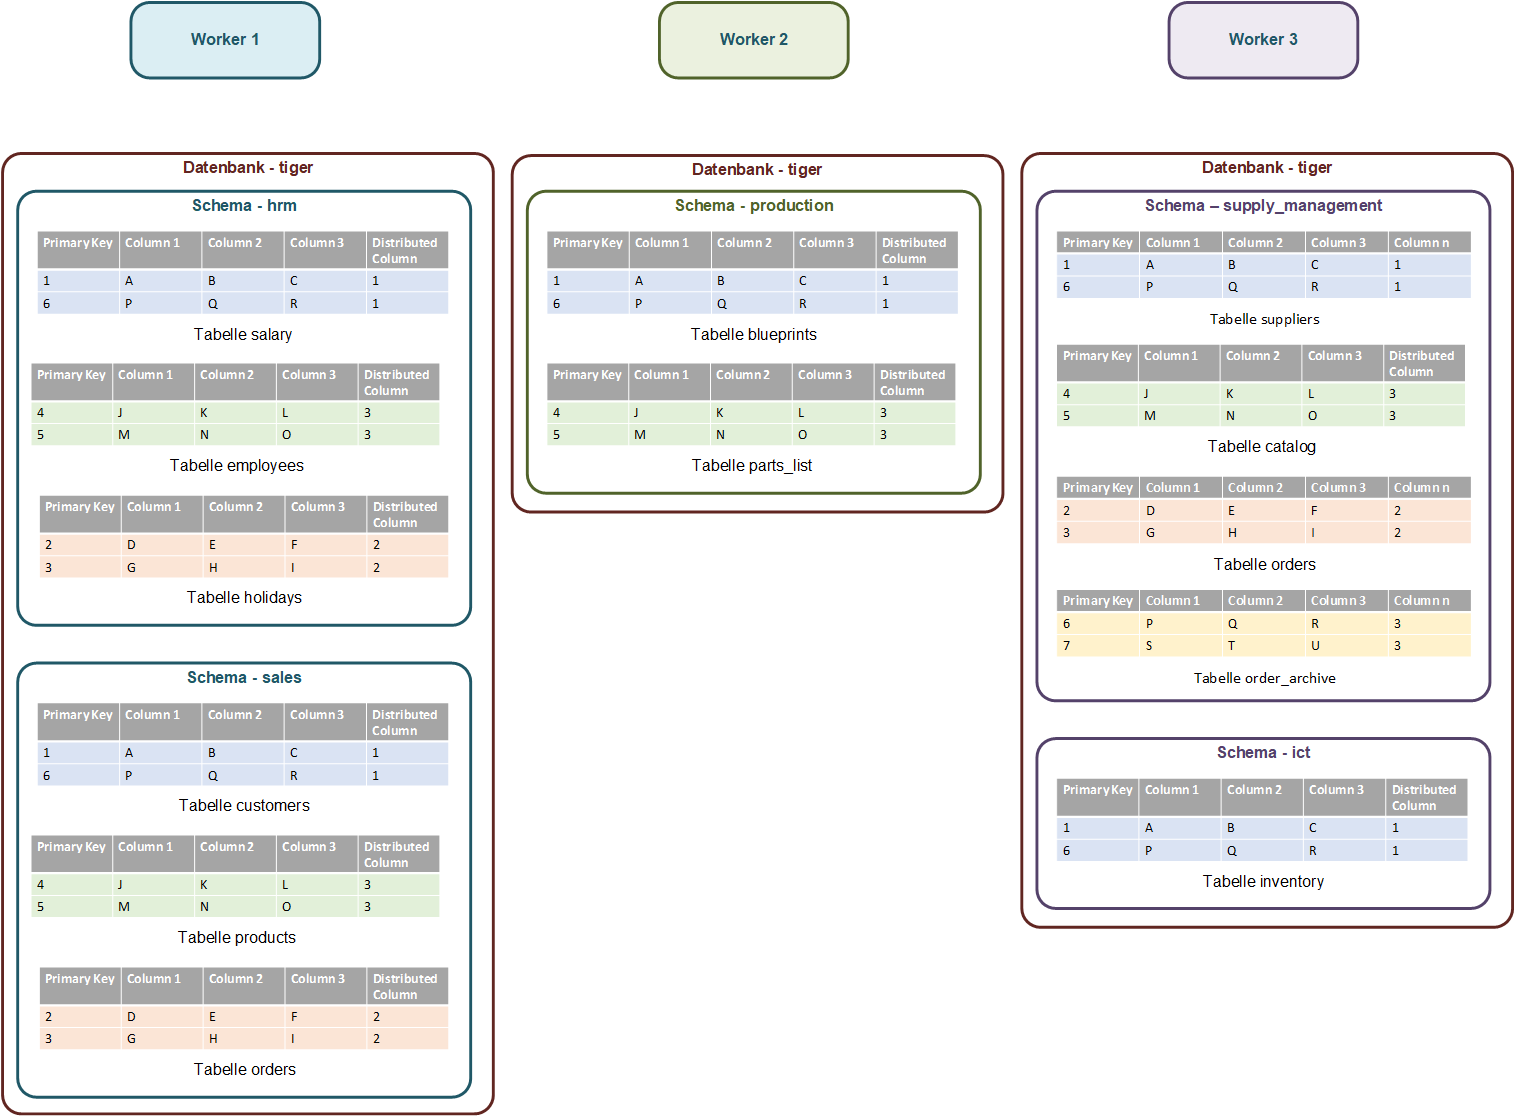
\includegraphics[width=0.8\linewidth]{source/implementation/evaluation/postgresql_ha_solutions/stackgres/citus_schema-based-sharding}
                \caption{Citus - Schema-Based-Sharding}
                \label{fig:citus_schema-based-sharding}
            \end{figure}
        \end{flushleft}
        \begin{flushleft}
            \textbf{Schlussfolgerung}\\
            Beide Sharding-Methoden haben eine grosse Schwäche.\\
            In Version 7.2 konnte noch ein Replikationsfaktor angegeben werden \cite{8W58EW47},\\
            ab Version 11 wurde auch diese Variante gestrichen und man konnte noch eine 1:1 Replikation auf einen Worker fahren \cite{JWYDYYWQ}.\\
            Spätestens mit Version 12 steht auch dies nicht mehr zur Verfügung, man muss eine Replication auf alle \Gls{Kubernetes} Nodes erzeugen.\\
%            Sie sind nicht vollständig ACID-Konform (\autoref{subsubsec:acid}) da Datenverlust entstehen kann, wenn ein Node wegfällt.
            Sie sind nicht vollständig ACID-Konform da Datenverlust entstehen kann, wenn ein Node wegfällt.
            Dies muss aber bei der Evaluation mit Hilfe von Tests noch bestätigt werden.
        \end{flushleft}
        \begin{flushleft}
            Die Shards müssen aber stand heute mit entsprechenden mit Replikation gesichert werden  \cite{4GDXA49I}.
            Daraus ergibt sich aber ein nicht zu vernachlässigbarer Mehraufwand, wenn man self-healing Nodes implementieren möchte.
            Jeder Node ist für sich genommen, eine eigene Zone. Um sicherzustellen, dass es zu keinem Datenverlust kommt,
            müsste jeder Shared-Node in eine der jeweiligen Zonen repliziert werden.
            Das heisst, es müssten \(Shard-Nodes^2 \) Replika-Nodes erstellt werden, hier ein Schematisches-Beispiel mit drei Shard-Nodes:
            \begin{figure}[H]
                \centering
                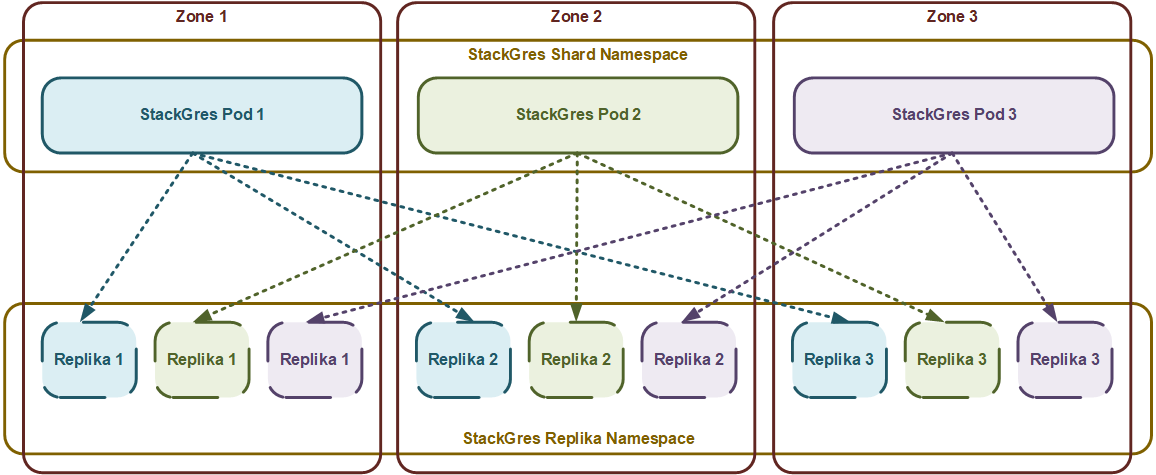
\includegraphics[width=0.8\linewidth]{source/implementation/evaluation/postgresql_ha_solutions/stackgres/stackgres_shard_replication}
                \caption{StackGres-Citus - Shard-Replikation}
                \label{fig:stackgres_shard_replication}
            \end{figure}
            Die Automation und nur schon die Konfiguration für das Mitskalieren, dürfte einiges an Zeit in Anspruch nehmen.\\
            Eine nicht unwesentliche Folge wäre ein starker Rückgang des Throughputs und Performance-Einbussen.
        \end{flushleft}
        \begin{flushleft}
            Alternativ kann ein klassischer Replika-Server verwendet werden, wo die ganze Datenbank gesichert wird.
            Bis alle Daten wieder in den StackGres-Citus-Cluster zurückgeholt wurden, das Re-Balancing abgeschlossen ist usw.,
            muss der ganze Cluster für die User unerreichbar sein, da dieser in dieser Zeit nicht mehr konsistent ist.
        \end{flushleft}
        \begin{flushleft}
            Dieser zweite Ansatz bietet zwar Vorteile beim Throughput, doch im Fehlerfall kann ein HA-Betrieb nur noch begrenzt garantiert werden.
        \end{flushleft}
    \end{flushleft}
\end{flushleft}
\begin{flushleft}
    \paragraph{Maintenance}
    Bei StackGres und Citus ist Citusdata, welches mittlerweile zu Microsoft gehört, sehr aktiv.\\
    Citusdata hält nicht nur die Community Standards ein, sondern Commited zyklisch und räumt alten Code regelmässig auf.\\
    Anders sieht es bei Ongres, dem Maintainer von StackGres, aus.\\
    Weder werden besonders viele Community Standards eingehalten, noch wird regelmässig Commited.\\
    Die Aktivitäten gingen in den letzten Jahren und Monaten zurück, was dazu führt, das immer wieder mal grössere Commits notwendig werden.\\
    Die genaue Analyse ist im \hyperref[subsec:maintenance_stackgres_citus]{Anhang - Maintenance} zu finden.
\end{flushleft}